\documentclass[a4j,12pt,]{jarticle}
 \usepackage[dvipdfmx]{graphicx}
 \usepackage{float}
 \usepackage{siunitx} %%SI単位系用
 \usepackage{amssymb, amsmath}
 \usepackage{ascmac,here,txfonts,txfonts}
\usepackage{listings,jlisting}
\usepackage[dvipdfmx]{color}
\lstset{%
  language={Python},
  basicstyle={\small},%
  identifierstyle={\small},%
  commentstyle={\small\itshape\color[rgb]{0,0.5,0}},%
  keywordstyle={\small\bfseries\color[rgb]{0,0,1}},%
  ndkeywordstyle={\small},%
  stringstyle={\small\ttfamily\color[rgb]{1,0,1}},
  frame={tb},
  breaklines=true,
  columns=[l]{fullflexible},%
  numbers=left,%
  xrightmargin=0zw,%
  xleftmargin=3zw,%
  numberstyle={\scriptsize},%
  stepnumber=1,
  numbersep=1zw,%
  lineskip=-0.5ex%
}
\begin{document}

{\noindent\small 第10回報告書 \hfill\today}
\begin{center}
  {\Large 日射量の計算式の計算精度の調査}
\end{center}
\begin{flushright}
  祖父江匠真 \\
\end{flushright}

\section{はじめに}
今回は, 相互相関の計算結果を改善するために, 現在使用している日射量の計算式の精度を調査した.

\section{日射量の計算値同士での相互相関}
図\ref{p1}に, 現在使用している日射量の計算式をもとに計算した値同士で求めた相互相関を示す.

\begin{figure}[H]
  \begin{center}
    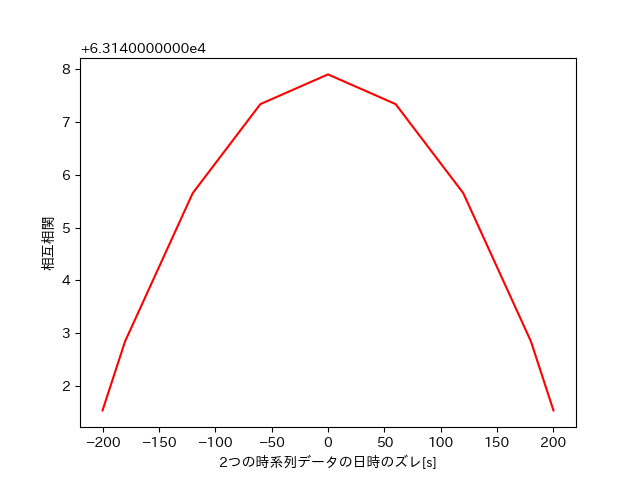
\includegraphics[width=160mm]{1.png}
    \caption{修正前の日射量の計算式によって求めた計算値同士での相互相関}
    \label{p1}
  \end{center}
\end{figure}

図\ref{p1}より, 1分ごとに相互相関の値が線形的に変化しているので, 日射量の計算式において秒の値が考慮されていないと推測し, 太陽の時角の式を確認したところ, 修正前の式(1)は秒の値が考慮されていなかった.

\begin{eqnarray}
  h = \frac{((時 + \frac{分}{60})-12)\pi}{12}+標準子午線からの経度差+E_q
\end{eqnarray}

そこで, 太陽の時角の式を, 時, 分だけでなく秒の値も組み込んだ式(2)に修正した上で, 再び計算値同士で相互相関を求めたものを図\ref{p2}に示す.
図\ref{p2}では, 秒単位で日射量が計算されるようになったことで, 図\ref{p1}とは異なり相互相関が非線形に変化している.

\begin{eqnarray}
  h = \frac{((時 + \frac{分}{60} + \frac{秒}{3600})-12)\pi}{12}+標準子午線からの経度差+E_q
\end{eqnarray}

\begin{figure}[H]
  \begin{center}
    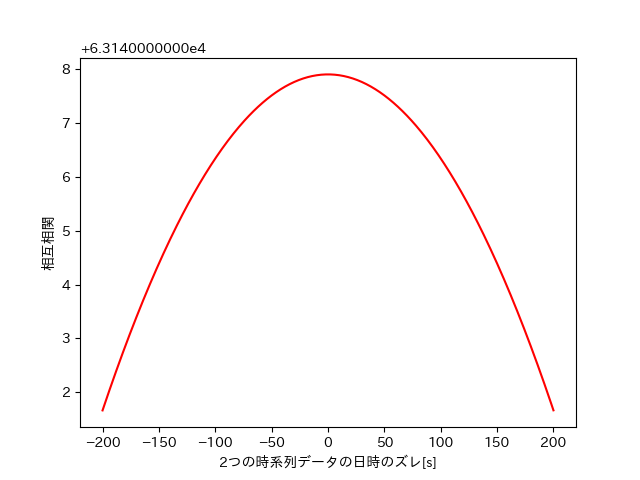
\includegraphics[width=160mm]{2.png}
    \caption{修正後の日射量の計算式によって求めた計算値同士での相互相関}
    \label{p2}
  \end{center}
\end{figure}

\section{修正後の日射量の式を用いた実測値と計算値の相互相関}
修正した太陽の時角の式(2)を使用して, 実測値との相互相関を計算し, 相互相関が最大になるラグが改善するか確認する.

相互相関の計算に使用する実測値の日射量データとして, 晴れの日の割合が多い2022年4月1日0時0分から2022年4月8日12時0分までの7.5日間と, 雨の日の割合が多い2022年4月23日0時0分から2022年4月30日12時0分までの7.5日間を使用する.

図\ref{p3}に, 晴れの日の割合が大きい期間の実測データを示す.

\begin{figure}[H]
  \begin{center}
    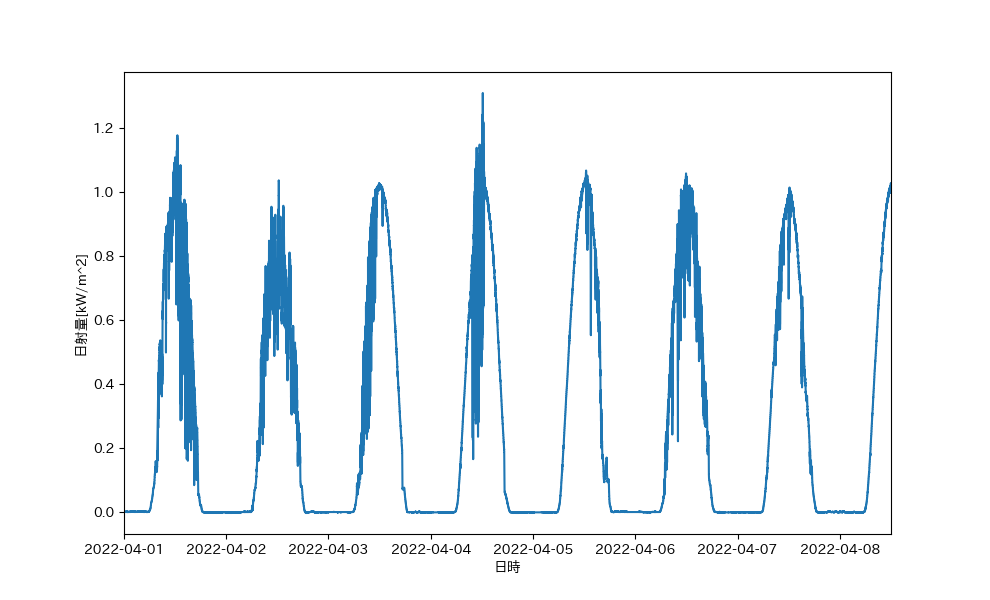
\includegraphics[width=160mm]{3.png}
    \caption{晴れの日の割合が大きい期間の実測データ}
    \label{p3}
  \end{center}
\end{figure}

図\ref{p4}に, 雨の日の割合が大きい期間の実測データを示す.

\begin{figure}[H]
  \begin{center}
    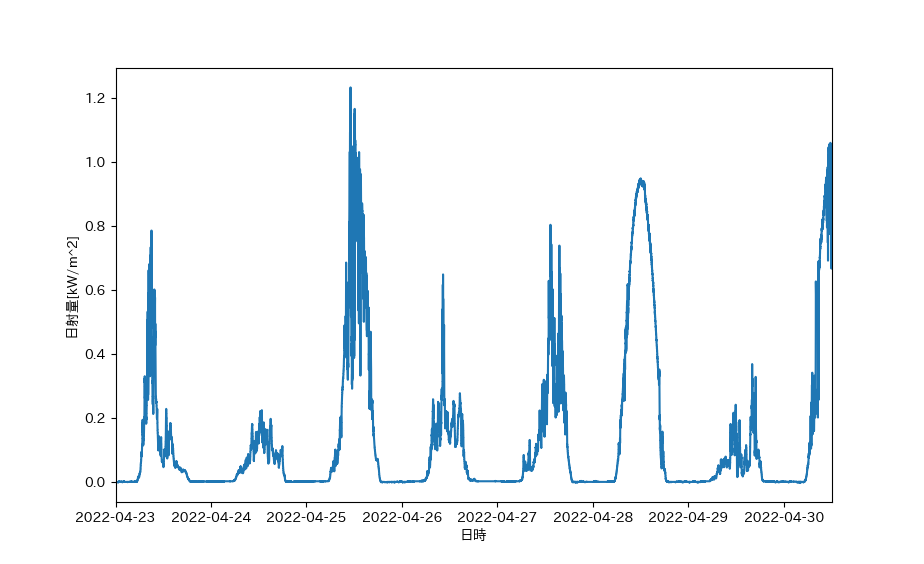
\includegraphics[width=160mm]{4.png}
    \caption{雨の日の割合が大きい期間の実測データ}
    \label{p4}
  \end{center}
\end{figure}

これらの実測値を使用して, 相互相関を求めた結果, 晴れの日の割合が大きい期間の実測データでは, 計算値の日時を実測値より1 \si{\second}遅らせた際に, 相互相関の値が最大となった.
また,  雨の日の割合が大きい期間の実測データでは, 計算値の日時を実測値より785 \si{\second}遅らせた際に, 相互相関の値が最大となった.

この結果から, 計算値と近い概形を持つ, 晴れの日の割合が大きい期間の実測データを使用して求めた相互相関が最大となるラグは32 \si{\second}から1 \si{\second}へと改善したが, 雨の日の割合が大きい期間の実測データを使用して求めた相互相関が最大となるラグは750 \si{\second}から785 \si{\second}へと改善しなかったことが分かった.

図\ref{p5}に晴れの日の割合が大きい期間の実測データと, 実測値より日時を1 \si{\second}遅らせた日射量の計算値を重ねてプロットしたものを示す.

\begin{figure}[H]
  \begin{center}
    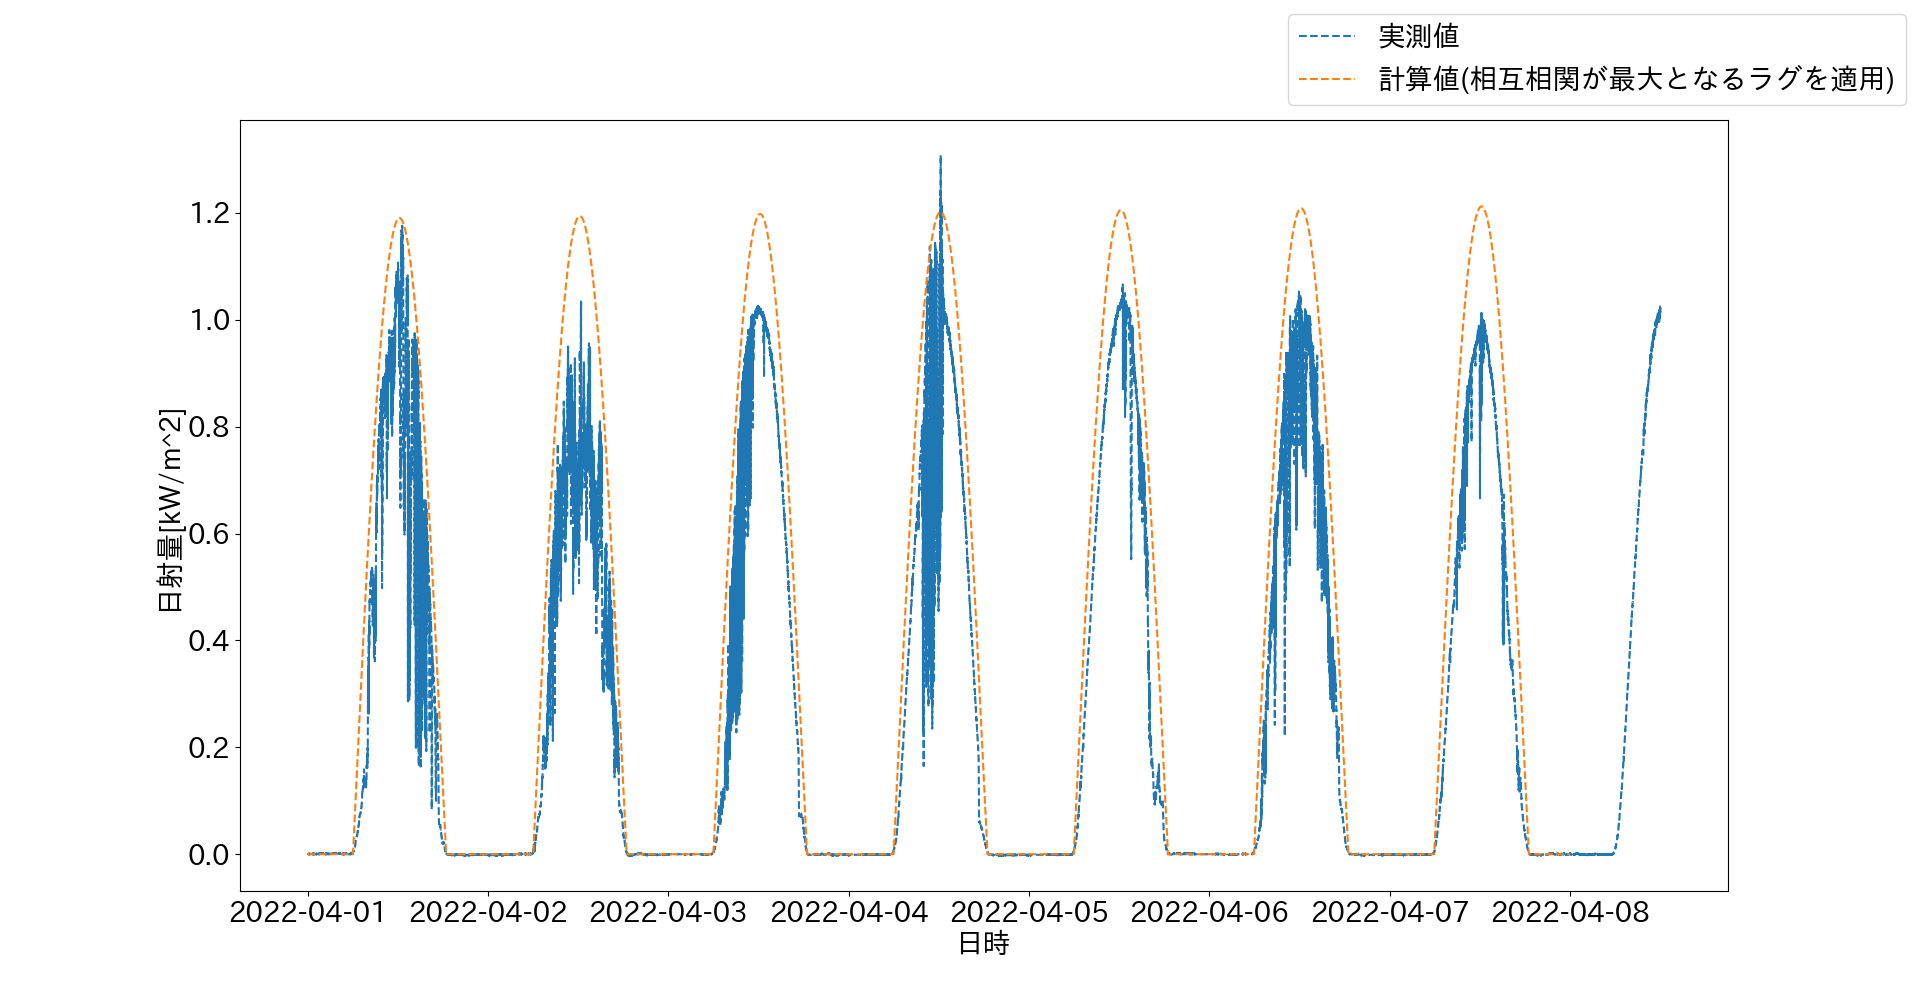
\includegraphics[width=160mm]{5.png}
    \caption{晴れの日の割合が大きい期間の実測データとラグを適用した計算値を重ねてプロットしたもの}
    \label{p5}
  \end{center}
\end{figure}


図\ref{p6}に雨の日の割合が大きい期間の実測データと, 実測値より日時を785 \si{\second}遅らせた日射量の計算値を重ねてプロットしたものを示す.

\begin{figure}[H]
  \begin{center}
    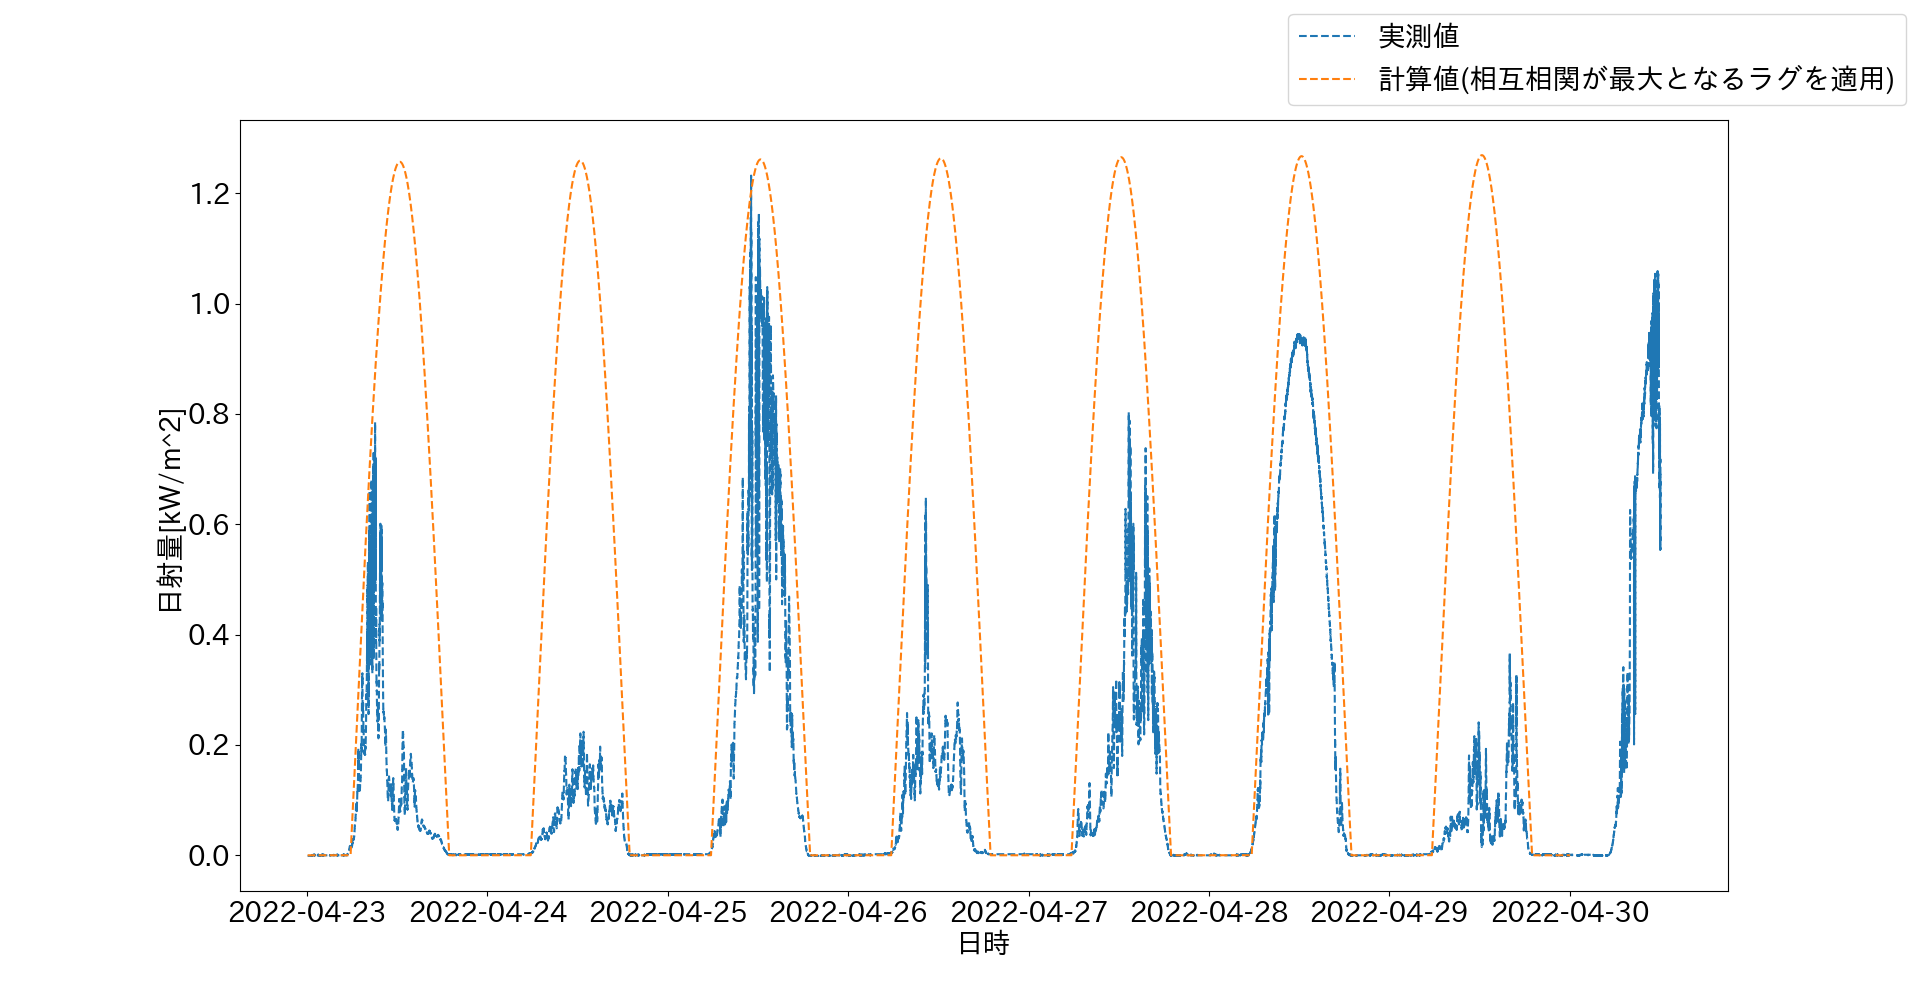
\includegraphics[width=160mm]{6.png}
    \caption{雨の日の割合が大きい期間の実測データとラグを適用した計算値を重ねてプロットしたもの}
    \label{p6}
  \end{center}
\end{figure}

\section{おわりに}
今回は, 相互相関の計算結果を改善するために, 現在使用している日射量の計算式の精度を調査した.

調査した結果, 修正前の太陽の時角の計算式は時, 分までしか考慮されておらず, 秒の値が切り捨てられていたので, 秒の値まで計算に含めた結果, 計算値に近い概形を持つ晴れの日の割合が大きい期間の実測データとの相互相関が最大となるラグが改善した.

\begin{thebibliography}{5}
  \bibitem{1}中川清隆,"太陽方位、高度、大気外日射量の計算", http://www.es.ris.ac.jp/~nakagawa/met\_cal/solar.html,参照 July 10, 2022.
  \bibitem{2}祖父江,"第7回報告書", teams内,参照 July 10, 2022.
\end{thebibliography}

\end{document}